\chapter*{Dodatak: Prikaz aktivnosti grupe}
		\addcontentsline{toc}{chapter}{Dodatak: Prikaz aktivnosti grupe}
		
		\section*{Dnevnik sastajanja}
		
		
		
		\begin{packed_enum}
			\item  sastanak
			
			\item[] \begin{packed_item}
				\item Datum: 15. listopad 2023.
				\item Prisustvovali: Luka Diktić, Luka Babić, Luka Žmak, Maja Mavračić, Mirta Posnjak, Dominik Poljak, Filip Sučić
				\item Teme sastanka:
				\begin{packed_item}
					\item  podjela poslova 
				
				\end{packed_item}
			\end{packed_item}
			
			\item  sastanak
			\item[] \begin{packed_item}
				\item Datum: 4. studenog 2023.
				\item Prisustvovali: Luka Diktić, Luka Babić, Luka Žmak, Maja Mavračić, Mirta Posnjak, Dominik Poljak, Filip Sučić
				\item Teme sastanka:
				\begin{packed_item}
					\item  odabir alata i tehnologija
					\item  definiranje funkcionalnih zahtjeva
				\end{packed_item}
			\end{packed_item}
			
			\item  sastanak
			\item[] \begin{packed_item}
				\item Datum: 20. prosinca 2023.
				\item Prisustvovali: Luka Diktić, Luka Babić, Luka Žmak, Maja Mavračić, Mirta Posnjak, Dominik Poljak, Filip Sučić
				\item Teme sastanka:
				\begin{packed_item}
					\item  podjela rada implementacije
					\item  podjela rada dokumentacije
				\end{packed_item}
			\end{packed_item}
			
			\item  sastanak
			\item[] \begin{packed_item}
				\item Datum: 10. siječnja 2024.
				\item Prisustvovali: Luka Diktić, Luka Babić, Luka Žmak, Maja Mavračić, Mirta Posnjak, Dominik Poljak, Filip Sučić
				\item Teme sastanka:
				\begin{packed_item}
					\item  završne podjele zadataka
					\item  podjela rada dokumentacije
				\end{packed_item}
			\end{packed_item}
			
			%
			
		\end{packed_enum}
		
		\eject
		\section*{Tablica aktivnosti}
		
			

			\begin{longtblr}[
					label=none,
				]{
					vlines,hlines,
					width = \textwidth,
					colspec={X[7, l]X[1, c]X[1, c]X[1, c]X[1, c]X[1, c]X[1, c]X[1, c]}, 
					vline{1} = {1}{text=\clap{}},
					hline{1} = {1}{text=\clap{}},
					rowhead = 1,
				} 
			
				\SetCell[c=1]{c}{} & \SetCell[c=1]{c}{\rotatebox{90}{\textbf{Luka Diktič}}} & \SetCell[c=1]{c}{\rotatebox{90}{\textbf{Maja Mavračić }}} &	\SetCell[c=1]{c}{\rotatebox{90}{\textbf{Mirta Posnjak }}} & \SetCell[c=1]{c}{\rotatebox{90}{\textbf{Filip Sučić }}} &	\SetCell[c=1]{c}{\rotatebox{90}{\textbf{Dominik Poljak }}} & \SetCell[c=1]{c}{\rotatebox{90}{\textbf{Luka Babić }}} &	\SetCell[c=1]{c}{\rotatebox{90}{\textbf{Luka Žmak }}} \\  
				Upravljanje projektom 		  &30  &  &  &  &7  &7  & \\ 
				Opis projektnog zadatka 	&  &  &  &  &  &  &5 \\ 
				
				Funkcionalni zahtjevi       &  &4  &4  &  &  &  &  \\ 
				Opis pojedinih obrazaca 	&  &5  &5  &  &  &  &5  \\ 
				Dijagram obrazaca 			&  &6  &  &  &  &  &  \\ 
				Sekvencijski dijagrami 		&  &  & 6 &  &  &  &  \\ 
				Opis ostalih zahtjeva 		&  &  &  &  &  &  &3  \\ 

				Arhitektura i dizajn sustava	 &7  &  &  &  &  &  &  \\ 
				Baza podataka				&  &  &  &2  &5  &5  &   \\ 
				Dijagram razreda 			&  &  &  &4  &  &  &   \\ 
				Dijagram stanja				&  &  &4  &  &  &  &  \\ 
				Dijagram aktivnosti 		&  &4  &  &  &  &  &  \\ 
				Dijagram komponenti			&  &  &  &  &  &5  &  \\ 
				Korištene tehnologije i alati 		&3  &  &  &  &  &  &  \\ 
				Ispitivanje programskog rješenja 	&3  &  &  &  &  &  &  \\ 
				Dijagram razmještaja			&  & 3 &  &  &  &  &  \\ 
				Upute za puštanje u pogon 		&  &  &  &  &  &  &4  \\  
				Dnevnik sastajanja 			&3  &  &  &  &  &  &  \\ 
				Zaključak i budući rad 		&  &  &  &  &  &4  &  \\  
				Popis literature 			&  &  &2  &  &  &  &  \\  
				&  &  &  &  &  &  &  \\ \hline 
				\textit{Dodatne stavke kako ste podijelili izradu aplikacije} 			&3  &  &  &  &  &  &  \\ 
				\textit{npr. izrada početne stranice} 				&3  &2  &2  &  &  &  &4  \\  
				\textit{izrada baze podataka} 		 			&  &  &  &  & 4 &4  & \\  
				\textit{spajanje s bazom podataka} 							& 5 &  &  &  &  &  &  \\ 
				\textit{back end} 							&10  &  &  & 6 &6  &6  &  \\  
				 							&  &  &  &  &  &  &\\ 
			\end{longtblr}
					
					
		\eject
		\section*{Dijagrami pregleda promjena}
		
		
		
		\begin{figure}[hbt!]
			\centering
			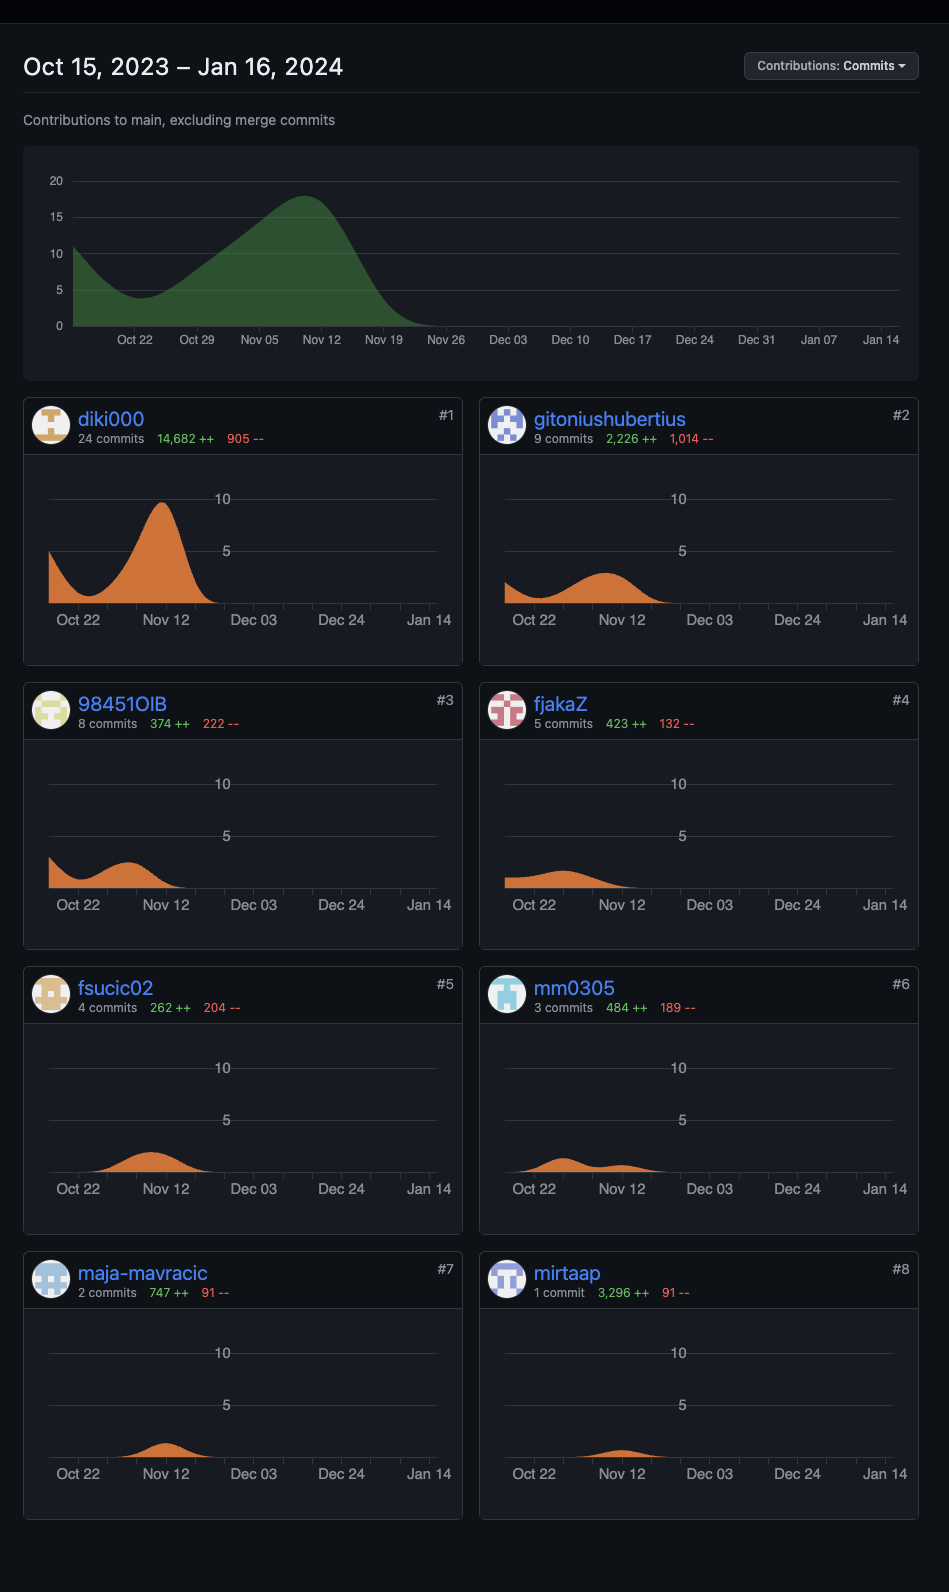
\includegraphics[width=0.7\linewidth]{slike/dijagrampregleda.png}
			\caption{prikaz aktivnosti na repozitoriju}
			\label{fig:dijagrampregleda}
		\end{figure}
		
		
		
		
		
	
		
	